\input{F:/Dropbox/Modeles_latex/Preambule_presentation_2013.tex}

%%%%%%%%%%%%%%%%%%%%%%%%%%%%%%%%%%%%%%%%%%%%%%%%%%%%%%%%%%%%%%%%%%%%%%%%%%%%%%
%Titre présentation Beamer
\title{Correction de l'exercice supplémentaire n° 1}  
\author{BAT 2}\institute{Lycée Jean Pierre Timbaud}
\date{}
%%%%%%%%%%%%%%%%%%%%%%%%%%%%%%%%%%%%%%%%%%%%%%%%%%%%%%%%%%%%%%%%%%%%%%%%%%%%%%%%%

%%%%%%%%%%%%%%%%%%%%%%%
%% DEBUT DU DOCUMENT %%
%%%%%%%%%%%%%%%%%%%%%%%

\begin{document}



%%%%%%%%%%%%%%%%%%%%%%%Page 1%%%%%%%%%%%%%%%%%%%%%%%%%%%%%%%%%%%%%%%%
%\begin{spacing}{1.2}

%Modèle propriété :
%\fbox{%
%   \begin{minipage}{\textwidth}
%   \textbf{\ul{Définition :}} \\
%   L'ensemble des matrices d'ordre $(n,p)$ à coefficients réels se note $\mathcal{M}_{n,p}(\R)$.
%   \end{minipage}%
%}


%Autre possibilité avec les packages de la partie ENCADRES
%\begin{bclogo}[couleur = gray!30 , arrondi = 0.1 ,logo = \bclampe , barre = snake , tailleOndu = 1.5]{Théorème}
%Soit $M$ la matrice de transition d'un graphe probabiliste.
%Soit $P_0$ la matrice ligne décrivant l'état initial.
%La matrice ligne $P_n$ décrivant l'état probabiliste à l'étape $n$ vérifie :
%$\bullet P_{n+1}=P_n\times M$
%$\bullet P_n=P_0\times M^n$
%\end{bclogo}
%%%%%%%%%%%%%%%%%%%%%%%%%%%%%%%%%%%%%%%%%%%%%%%%%%%%%%%%%%%%
\begin{frame}
 \titlepage
\end{frame}
%%%%%%%%%%%%%%%%%%%%%%%%%%%%%%%%%%%%%%%%%%%%%%%%%%%%%%%%%%%%%
\section{Question a)}
\begin{frame}{Question a)}

\begin{itemize}
 	
	\item Je n'ai pas le même énoncé que vous...
	
	\item Dans mon livre, la question porte sur l'année 2006.
	
	\item Notons $(u_n)$ la production de bicyclettes pour la consommation intérieure à l'année $2005+n$ (ce qui signifie que $u_0=2 000 000$) et $(v_n)$ la production pour l'exportation à la même année ($v_0=250 000$).
	
	\item Notons $(w_n)$ la production totale de bicyclette à l'année $2005+n$.
	
	\item On a donc, pour tout $n \in \N$, $w_n=u_n+v_n$.
	
	\item $u_1=2 000 000 \times 1,1 = 2 200 000$, $v_1=250 000 \times 1,32 = 330 000$.
	
	\item Donc, la production totale pour 2006 doit être de :
	
	\item $w_1=u_1+v_1=2 200 000+330 000=2 530 000$ bicyclettes.
	
	\end{itemize}
\end{frame}


%%%%%%%%%%%%%%%%%%%%%%%%%%%%%%%%%%%%%%%%%%%%%%%%%%%%%%%%%%%%%%%%%
\section{Question b)}

\begin{frame}[allowframebreaks]{Question b)}


\label{départ}

\pause
\begin{block}{Un bloc normal}
On cherche $w_8=u_8+v_8$.
\end{block}	

\pause	
\setbeamertemplate{blocks}[rounded]
[shadow=true]	
	\begin{block}{Un bloc ombré}
On cherche $w_8=u_8+v_8$.
\end{block}

\begin{itemize}		
	\item La suite $(u_n)$ est la suite géométrique de premier terme $u_0=2 000 000$ et de raison $b=1,1$.
		
	\item La suite $(v_n)$ est la suite géométrique de premier terme $v_0=250 000$ et de raison $b=1,32$.
	
	\item Ainsi, pour tout $n \in \N$, on a :
	
	\item $u_n=u_0 \times a^n=2 000 000 \times 1,1^n$ et $v_n=v_0 \times b^n=250 000 \times 1,32^n$.
	
	\item Donc, $w_8=u_8+v_8=2 000 000 \times 1,1^8 + 250 000 \times 1,32^8 \approx 6 591 438$.
	
	\item Pour satisfaire la demande, la production devra être de 6 591 438 bicyclettes en 2013.
	
	\item\textcolor{orange}{Si on utilise la fonction $\ln$ pour résoudre l'inéquation (*), on écrira :}
		
	\pause\item\textcolor{orange}{$1,2^n > 8 \Leftrightarrow \ln \left( 1,2^n\right) > \ln (8) \Leftrightarrow n \ln (1,2) > \ln (8)$\\
	$\Leftrightarrow n > \dfrac{\ln(8)}{\ln(1,2)}$}
		
	\pause\item\textcolor{orange}{Or $\dfrac{\ln(8)}{\ln(1,2)} \approx 11,4$.}
	
	\pause\item\textcolor{orange}{On obtient donc la même conclusion.}
	
	\end{itemize}
\end{frame}


%%%%%%%%%%%%%%%%%%%%%%%%%%%%%%%%%%%%%%%%%%%%%%%%%%%%%%%%%%%%%

\section{Question c)}

\begin{frame}{Question c)}

\begin{itemize}
 	
	\item On cherche $n$ pour que $v_n > u_n$, c'est-à-dire
		
	\item $250 000 \times 1,32^n > 2 000 000 \times 1,1^n$.
		
	\item Or, $250 000 \times 1,32^n > 2 000 000 \times 1,1^n$\\ $\Leftrightarrow \dfrac{1,32^n}{1,1^n} > \dfrac{2 000 000}{250 000} \Leftrightarrow \left( \dfrac{1,32}{1,1}\right)^n > 8 \Leftrightarrow 1,2^n > 8$. (*)
	
	\item Nous n'avons pas, pour l'instant, de formule permettant de trouver l'entier $n$ qui convient.
	
	\item En essayant quelques valeurs de $n$, on obtient :
	
	\item $1,2^{11} \approx 7,4$ et $1,2^{12} \approx 8,9$.
	
	\item C'est donc à partir de la $12^{\text{ème}}$ année (après 2005, c'est-à-dire en 2017) que l'exportation dépassera pour la première fois la consommation intérieure.
	
	\end{itemize}
\end{frame}


%%%%%%%%%%%%%%%%%%%%%%%%%%%%%%%%%%%%%%%%%%%%%%%%%%%%%%%%%%%%%

\section{Avec la fonction ln}



\begin{frame}
%:-+-+-+-+- Engendré par : http://math.et.info.free.fr/TikZ/TableauxVariations/
\begin{center}
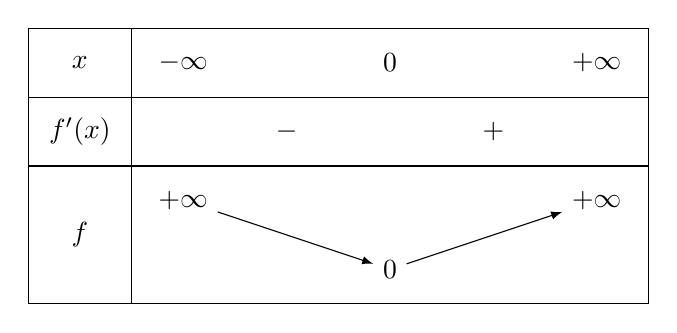
\begin{tikzpicture}[scale=0.875]
% Styles 
\tikzstyle{cadre}=[thin]
\tikzstyle{fleche}=[->,>=latex,thin]
\tikzstyle{nondefini}=[lightgray]
% Dimensions Modifiables
\def\Lrg{1.5}
\def\HtX{1}
\def\HtY{0.5}
% Dimensions Calculées
\def\lignex{-0.5*\HtX}
\def\lignef{-1.5*\HtX}
\def\separateur{-0.5*\Lrg}
% Largeur du tableau
\def\gauche{-1.5*\Lrg}
\def\droite{4.5*\Lrg}
% Hauteur du tableau
\def\haut{0.5*\HtX}
\def\bas{-2.5*\HtX-2*\HtY}
% Ligne de l'abscisse : x
\node at (-1*\Lrg,0) {$x$};
\node at (0*\Lrg,0) {$-\infty$};
\node at (2*\Lrg,0) {$0$};
\node at (4*\Lrg,0) {$+\infty$};
% Ligne de la dérivée : f'(x)
\node at (-1*\Lrg,-1*\HtX) {$f'(x)$};
\node at (0*\Lrg,-1*\HtX) {$$};
\node at (1*\Lrg,-1*\HtX) {$-$};
\node at (2*\Lrg,-1*\HtX) {$$};
\node at (3*\Lrg,-1*\HtX) {$+$};
\node at (4*\Lrg,-1*\HtX) {$$};
% Ligne de la fonction : f(x)
\node  at (-1*\Lrg,{-2*\HtX+(-1)*\HtY}) {$f$};
\node (f1) at (0*\Lrg,{-2*\HtX+(0)*\HtY}) {$+\infty$};
\node (f2) at (2*\Lrg,{-2*\HtX+(-2)*\HtY}) {$0$};
\node (f3) at (4*\Lrg,{-2*\HtX+(0)*\HtY}) {$+\infty$};
% Flèches
\draw[fleche] (f1) -- (f2);
\draw[fleche] (f2) -- (f3);
% Encadrement
\draw[cadre] (\separateur,\haut) -- (\separateur,\bas);
\draw[cadre] (\gauche,\haut) rectangle  (\droite,\bas);
\draw[cadre] (\gauche,\lignex) -- (\droite,\lignex);
\draw[cadre] (\gauche,\lignef) -- (\droite,\lignef);
\end{tikzpicture}
\end{center}
%:-+-+-+-+- Fin

%:>>>>> code du tableau à ré-injecter
%[
%	["x", "f'(x)", "Variatiosn \\par de \\par f"],
%	["-\\infty", "", "-", "+\\infty"],
%	["0", "", "+", "0"],
%	["+\\infty", "", "?", "+\\infty"]
%]

\end{frame}

\begin{frame}
\begin{minipage}{0.45\linewidth}
bonjour

\includegraphics[width=0.3\textwidth]{fig1}
\end{minipage}
\hspace{0.05\linewidth}
\begin{minipage}{0.45\linewidth}
au revoir

\hyperlink{départ}{\beamerskipbutton{Départ}}

\href{run:geogebra.ggb}{\beamerskipbutton{Ficher Geogebra}}

\includegraphics[width=0.3\textwidth]{fig1}
\end{minipage}
\end{frame}

%%%%%%%%%%%%%%%%%%%%%%%%%%%%%%%%%%%%%%%%%%%%%%%%%%%%%%%%%%%%

%\end{spacing}

%%%%%%%%%%%%%%%%%%%%%%%%%%%%%%%%%%%%%%%%%%%%%%%%%%%%%%%%%%%%
%%%%%%%%%%%%%%%%%%%%%
%% FIN DU DOCUMENT %%
%%%%%%%%%%%%%%%%%%%%%
\end{document}